\clearpage
\sffamily
{\bfseries\color[rgb]{0.4,0.4,0.4}
Part B: Goal-Kick from Moving Ball}

\bigskip

The goal of the goal-kick from a moving ball challenge is to kick a moving ball into the goal. A ramp will be placed in a fixed position on the extension of the goal area line, such that a ball released from the ramp will travel parallel to the goal line towards the center of the field. The height of the ramp is adjustable and determines the initial velocity of the ball. Teams may place one robot anywhere on the field. After the ball has been released, the robot must make contact with it before the ball comes to a stop, otherwise the trial is unsuccessful.
If after the ball contact the ball enters the goal, the trial is successful. Otherwise the trial is partially successful. Teams are first ranked by the release height of the ball from the ramp for successful trials and then by the shortest distance between the ball and the goal for partially successful trials.


\begin{figure}[h]
\begin{center}
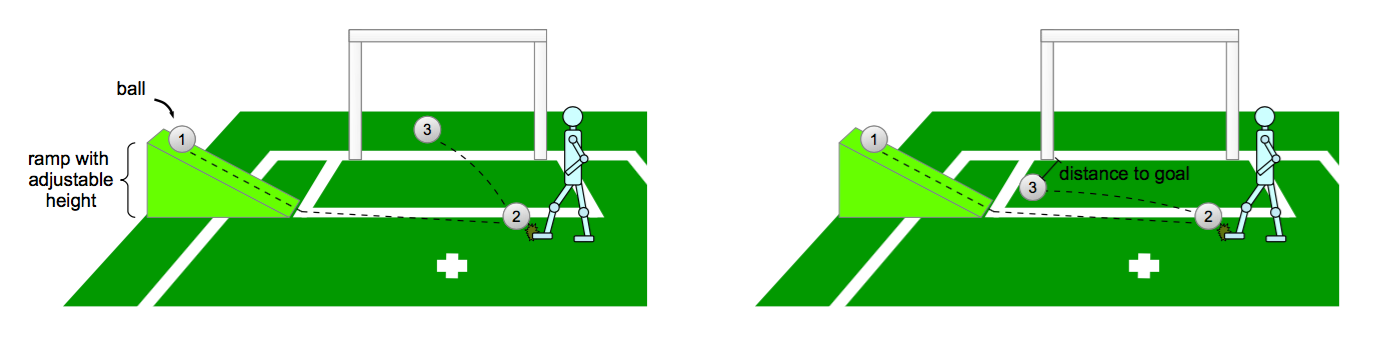
\includegraphics[width=\textwidth]{img/moving-ball.png}
\caption{Successful (left) and partially successful (right) goal-kick from a moving ball challenges.}
\end{center}
\end{figure}